\documentclass[14pt]{extarticle}
\usepackage[]{geometry}
\usepackage{graphicx}
\usepackage{pgfplots}
\usepackage{mathtools}
\usepackage[thinc]{esdiff}
\usepackage{bbm}
\usepgfplotslibrary{fillbetween}
\pgfplotsset{width=10cm,compat=1.9}

\title{MA-105 Tutorial-5 -- Solutions}
\author{Daksh Maahor}
\date{August 2025}

\begin{document}

\maketitle

\begin{enumerate}

%%%%%%%%%%%%%%%%%%%%%%%%%%%%%%%%%%%%%%%%%%%%%%%%%%%%%%%%%%%%
\item \textbf{Find the volume of the solid obtained by revolving the given shaded region about the x-axis.}

\begin{center}
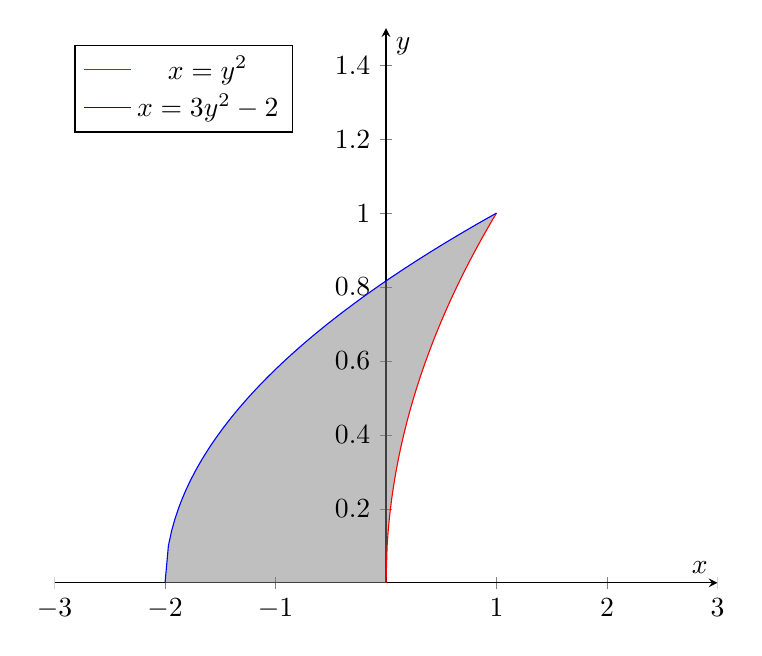
\begin{tikzpicture}
    \begin{axis}[
        axis lines = middle,
        xlabel = $x$,
        ylabel = {$y$},
        legend pos=north west,
        xmin=-3,
        xmax=3,
        ymax=1.5
    ]
    \addplot [name path=curve1, domain=0:1, samples=100, color=red]{sqrt(x)};
    \addlegendentry{$x = y^2$}
    \addplot [name path=curve2, domain=-2:1, samples=100, color=blue]{sqrt((x+2)/3)};
    \addlegendentry{$x = 3y^2 - 2$}
    \addplot [color=gray, opacity=0.5] fill between[of = curve1 and curve2];
    \end{axis}
\end{tikzpicture}
\end{center}

\textbf{Solution : }

The given region is bounded by the curves:
\[x = y^2, \quad x = 3y^2 - 2\]
Their intersection points occur when:
\[y^2 = 3y^2 - 2 \implies 2y^2 = 2 \implies y = \pm 1\]

The limits for $y$ are from $0$ to $1$. Revolving around the x-axis means each horizontal strip at height $y$ generates a shell of radius $y$ and thickness $dy$. Since our equations are in terms of $y$, we use the shell method:
\begin{align*}
V &= 2\pi \int_{0}^{1} y( x_{right} - x_{left} ) dy\\ &= 2\pi \int_{0}^{1} y[(y^2)-(3y^2 - 2)] dy \\&= 2\pi \int_{0}^{1} y(2 - 2y^2) dy \\&=2\pi\left(y^2-\frac{y^4}{2}\right)\Biggr|_{0}^{1} \\ &= \pi
\end{align*}
\[
\boxed{V = \pi}
\]

\newpage

%%%%%%%%%%%%%%%%%%%%%%%%%%%%%%%%%%%%%%%%%%%%%%%%%%%%%%%%%%%%
\item \textbf{Prove that if $f:[a,b] \to \mathbbm{R}$ is continuous, then $\exists c \in [a,b]$ such that}
\[\int_a^b f(x)dx = (b-a)f(c)\]
\textbf{and deduce that} $\diff{}{x}\int_a^x f(t)dt = f(x)$.

\textbf{Solution :}

Since $f$ is continuous on $[a,b]$, it attains its maximum $M$ and minimum $m$. By the properties of integrals:
\[m(b-a) \leq \int_a^b f(x)dx \leq M(b-a)\]
Dividing both sides by $(b-a)$ gives:
\[m \leq \frac{1}{b-a}\int_a^b f(x)dx \leq M\]
By the Intermediate Value Theorem, there exists $c \in [a,b]$ such that:
\[f(c) = \frac{1}{b-a}\int_a^b f(x)dx\]
Multiplying both sides by $(b-a)$, we obtain:
\[\boxed{\int_a^b f(x)dx = (b-a)f(c)}\]

To deduce $\diff{}{x}\int_a^x f(t)dt = f(x)$, define $F(x) = \int_a^x f(t)dt$. For any $h>0$,
\[\frac{F(x+h)-F(x)}{h} = \frac{1}{h}\int_x^{x+h} f(t)dt\]
By the Mean Value Theorem for integrals, there exists $c_h \in [x,x+h]$ such that:
\[\frac{F(x+h)-F(x)}{h} = f(c_h)\]
Taking $h\to0$, continuity of $f$ implies $c_h\to x$ and thus:
\[\boxed{F'(x) = f(x)}\]

\newpage

%%%%%%%%%%%%%%%%%%%%%%%%%%%%%%%%%%%%%%%%%%%%%%%%%%%%%%%%%%%%
\item \textbf{Prove that the set $\left\{(x,y)\mid \frac{x^2}{44}-\frac{y^2}{37}<1\right\}$ is open.}

\textbf{Solution :}

Let
\[
g(x,y)=\frac{x^2}{44}-\frac{y^2}{37},\qquad (x,y)\in\mathbbm{R}^2,
\]
and let
\[
S=\{(x,y)\in\mathbbm{R}^2\mid g(x,y)<1\}.
\]
Take an arbitrary point \(p=(x_0,y_0)\in S\). Then \(g(p)<1\); set
\[
\varepsilon := 1 - g(p) > 0.
\]

We claim there exists \(\delta>0\) such that for every point \(q=(x,y)\) with \(\|(x,y)-(x_0,y_0)\|<\delta\) we have \(g(q)<1\). This will show the open ball \(B_\delta(p)\subset S\) and hence that \(p\) is an interior point; since \(p\) was arbitrary, \(S\) is open.

To prove the claim use the limit (continuity) of \(g\) at \(p\). Note that \(g\) is a polynomial in \(x,y\), so
\[
\lim_{(x,y)\to(x_0,y_0)} g(x,y) = g(x_0,y_0).
\]
By the \(\varepsilon\)-\(\delta\) definition of a limit, since \(|g(x_0,y_0)-1|=\varepsilon>0\), there exists \(\delta>0\) such that
\[
|g(x,y)-g(x_0,y_0)|<\varepsilon \quad\text{whenever}\quad \|(x,y)-(x_0,y_0)\|<\delta.
\]
For such \((x,y)\) we get
\[
g(x,y) < g(x_0,y_0) + \varepsilon = g(x_0,y_0) + (1-g(x_0,y_0)) = 1.
\]
Hence every point \(q\) in the ball \(B_\delta(p)\) satisfies \(g(q)<1\), so \(B_\delta(p)\subset S\). Therefore \(p\) is an interior point of \(S\). As this holds for every \(p\in S\), the set \(S\) is open.

%%%%%%%%%%%%%%%%%%%%%%%%%%%%%%%%%%%%%%%%%%%%%%%%%%%%%%%%%%%%
\item \textbf{Is the set $\left\{(x, y)\mid \frac{x^2}{4}+\frac{y^2}{9}<1\right\}$ convex?}

\textbf{Solution :}

Let $S$ be the given set. For any two points $(x_1, y_1), (x_2, y_2)\in S$, we must show that every point on the line segment joining them is also in $S$.

Consider $(x,y)=t(x_1,y_1)+(1-t)(x_2,y_2)$, where $0\le t\le1$. Then:
\[\frac{x^2}{4}+\frac{y^2}{9} \le t\left(\frac{x_1^2}{4}+\frac{y_1^2}{9}\right)+(1-t)\left(\frac{x_2^2}{4}+\frac{y_2^2}{9}\right) < t+(1-t)=1\]
using convexity of the quadratic function. Hence the set is convex.
\[\boxed{S\text{ is convex.}}\]

%%%%%%%%%%%%%%%%%%%%%%%%%%%%%%%%%%%%%%%%%%%%%%%%%%%%%%%%%%%%
\item \textbf{Prove that a polynomial in two variables is a continuous function.}

\textbf{Solution :}

Let $p(x,y)=\sum_{i,j} a_{ij}x^iy^j$. Each monomial $x^iy^j$ is continuous as it is a product of continuous functions. A finite linear combination of continuous functions is continuous, hence $p(x,y)$ is continuous on $\mathbbm{R}^2$.
\[\boxed{p\text{ is continuous everywhere.}}\]

\newpage

%%%%%%%%%%%%%%%%%%%%%%%%%%%%%%%%%%%%%%%%%%%%%%%%%%%%%%%%%%%%
\item \textbf{Prove that if $f(x, y)$ is continuous, then the level set }
\[
L_c = \{(x, y) \in \mathbbm{R}^2 \mid f(x, y) = c\}
\]
\textbf{is closed.}

\textbf{Solution :}

Let $(x_n, y_n)$ be a sequence in $L_c$ that converges to some point $(x_0, y_0) \in \mathbbm{R}^2$. We want to show that $(x_0, y_0) \in L_c$, that is, $f(x_0, y_0) = c$.

Since $f$ is continuous at $(x_0, y_0)$, we have
\[
\lim_{n \to \infty} f(x_n, y_n) = f\big(\lim_{n \to \infty} (x_n, y_n)\big) = f(x_0, y_0).
\]

But each $(x_n, y_n) \in L_c$, so $f(x_n, y_n) = c$ for all $n$. Therefore,
\[
\lim_{n \to \infty} f(x_n, y_n) = \lim_{n \to \infty} c = c.
\]

Combining the two limits, we get
\[
f(x_0, y_0) = c.
\]

Hence, $(x_0, y_0) \in L_c$, proving that $L_c$ contains all its limit points. By definition, this means $L_c$ is closed.

\[
\boxed{L_c \text{ is closed.}}
\]

\newpage

%%%%%%%%%%%%%%%%%%%%%%%%%%%%%%%%%%%%%%%%%%%%%%%%%%%%%%%%%%%%
\item \textbf{Sketch the level sets of $f(x,y,z)=x^2+y^2-z^2$.}

We have $f(x,y,z)=k \implies x^2+y^2-z^2=k$.

- For $k>0$, we get a \textbf{two-sheeted hyperboloid}.
- For $k=0$, we get a \textbf{double cone}.
- For $k<0$, we get a \textbf{one-sheeted hyperboloid}.

\begin{center}
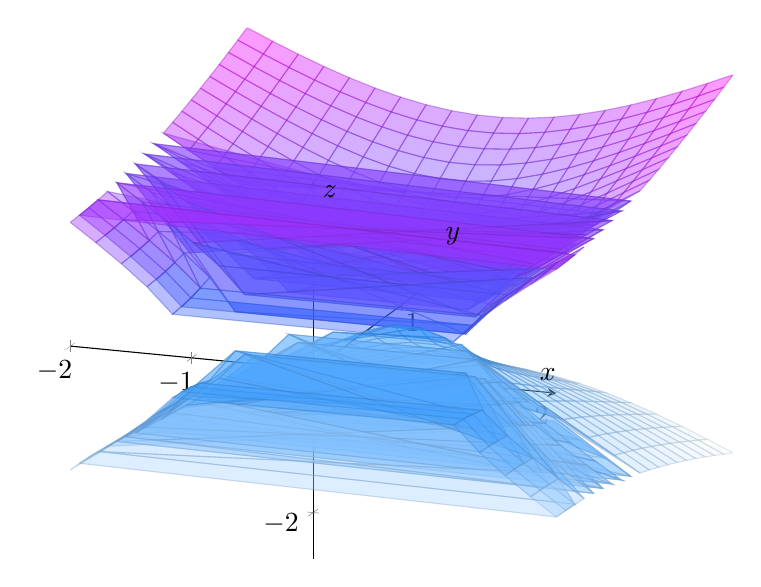
\begin{tikzpicture}[scale=1]
\begin{axis}[
    view={20}{20},
    xlabel=$x$, ylabel=$y$, zlabel=$z$,
    axis lines=center,
    domain=-2:2,
    samples=20,
    colormap/cool
]
\addplot3[surf,opacity=0.4,domain=-2:2,y domain=0:2,samples=20]{sqrt(x^2+y^2-1)};
\addplot3[surf,opacity=0.4,domain=-2:2,y domain=0:2,samples=20]{-sqrt(x^2+y^2-1)};
\end{axis}
\end{tikzpicture}
\end{center}

These represent the level surfaces for $f(x,y,z)=1$ and $f(x,y,z)=-1$, respectively.

\end{enumerate}

\end{document}
